\section{Komponenten}

%5.1 Server Software
\subsection{Komponente \textit{ServerSoftware}}
\begin{figure}[H]
\centering
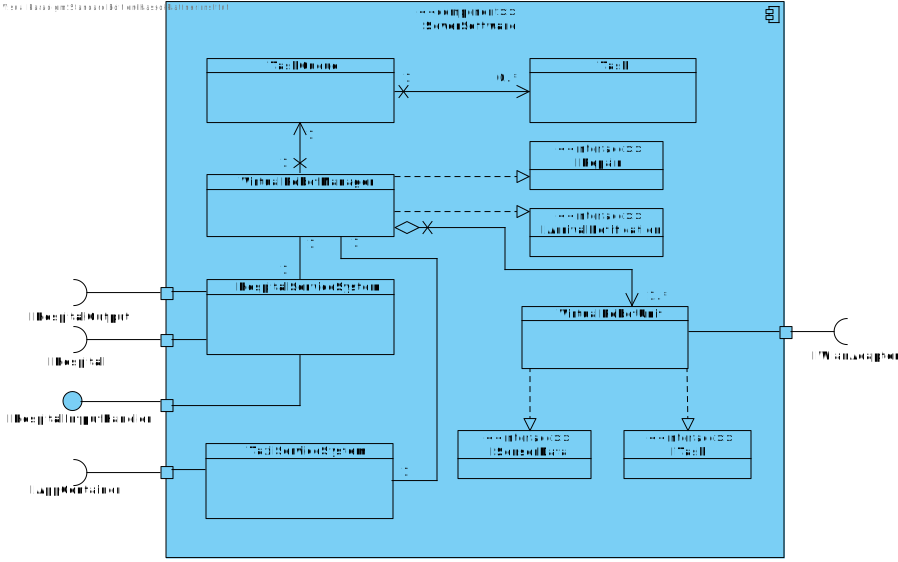
\includegraphics[height=0.7\textwidth, angle=90]{img/2-Entwurf-5-ServerSoftware}
\caption{\emph{ServerSoftware}-Komponentendiagramm}
\label{KomponentenStruktur1}
\end{figure}
Abbildung \ref{KomponentenStruktur1} zeigt ein Komponentendiagramm von \emph{ServerSoftware}. 
Diese Komponente umfasst vier Klassen: \textit{TaskSystem}, \textit{Destination}, \textit{RobotControlSystem}, \textit{VirtualRobot} und \textit{HospitalServiceSystem}.


Das \textit{TaskSystem} verwaltet die \textit{Tasks} und liefert Information über diese. 
Die Klasse \textit{Destination} ist die Klasse
der Aufgaben, die vom \textit{TaskSystem} verwaltet werden. 
Das \textit{RobotControlSystem} verteilt die \textit{Tasks} auf die \textit{Robots}.
Dabei findet die Auswahl anhand der zurückgegebenen \textit{SensorData} der einzelnen \textit{Robots} statt. 
Bei \textit{VirtualRobot} handelt
es sich um eine Kapselung der Kommunikation mit den \textit{Robots}. 
Hier werden alle von der Komponente \textit{Robot} bereitgestellten
\textit{Interfaces} implementiert.
%5.1 Robot Software
\subsection{Komponente \textit{RobotSoftware}}
\begin{figure}[H]
\centering
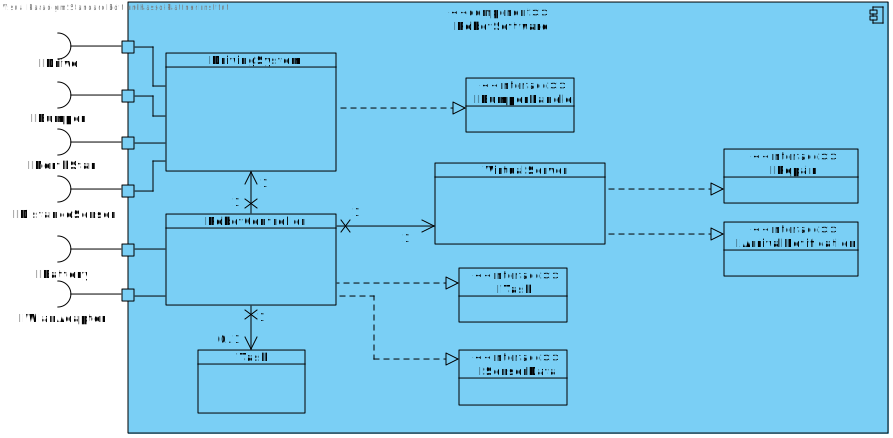
\includegraphics[width=1\textwidth]{img/2-Entwurf-5-RobotSoftware}
\caption{\emph{RobotSoftware}-Komponentendiagramm}
\label{KomponentenStruktur2}
\end{figure}
In Abbildung \ref{KomponentenStruktur2} ist das Komponentendiagramm der Komponente \textit{RobotSoftware} dargestellt. 
Die Komponente enthält drei Klassen: \textit{DrivingSystem}, \textit{RobotController} und \textit{Task}.


Das \textit{DrivingSystem} stellt eine Abstraktion der Hardware dar und wird dazu genutzt, Ziele anzufahren und dabei,
falls nötig, Hindernisse zu umfahren. 
Dazu greift es auf die von der Hardware bereitgestellten Interfaces zurück.
Um auf Kollisionen reagieren zu können, implementiert das \textit{DrivingSystem} die Schnittstelle \textit{IBumperHandler}.
Der \textit{RobotController} stellt dem Server das Interfaces \textit{ISensorData} zur Verfügung und verwaltet den gerade
zu absolvierenden \emph{Task}. 
Zur Messwertübermittlung greift er zum einen auf das \textit{DrivingSystem} und zum anderen auf das
von der Hardware angebotenen Interface \textit{IBattery} zu.
